\chapter{Texture Mapping}
Grundidee vom Texturemapping ist es, dass man Bilder etwas realistischer gestalten kann, ohne dass man mehr Polygone hinzufügen muss. Hat man z.B. in einer Szene ein Bild an der Wand, so kann z.B. einfach ein Rechteck als Polygon genommen werden und jetzt grob gesagt ein PNG darüber gespannt werden. Dann hat man ein detailliertes Bild, ohne von den darunterliegenden Polygonen abhängig zu sein. Oder siehe Minecraft - Blöcke mit Texturen darauf.

\section{Prozedurale Texturen}
Wenn man z.B. eine Holzkiste hat, so ist es nicht möglich oder zu mühsam, eine exakte PNG Datei zu erstellen. Bei Blöcken in Minecraft mag das ja gehen, aber sobalds dann komplexere Objekte werden, kann man auf prozedural generierte Textren zurückgreifen. Dabei werden die Holzstrukturen, oder Marmor usw dynamisch generiert und es ist egal, wie gross das Objekt schlussendlich ist.

\section{Textur Korrdinaten}
Der Pixel x,y vom Bild ist dann schlussendlich wo auf dem Objekt? Dsa macht man mit Transformationen - ist ja klar. Wie aber genau?
\subsection{Kugel}
Wenn wir eine Kugel haben, z.B. wie die Erde ja eine ist, dann können wir mit Längen und Breiten Angaben arbeiten. Das heisst, dass wir die Winkel \(\phi\) und \(\theta\) frei wählen können, mit der folgenden Formel kriegen wir dann alle möglichen Koordinaten der Kugel:

\begin{displaymath}
x = r\cdot cos \theta \cdot  sin \phi
\end{displaymath}
\begin{displaymath}
y = r\cdot sin \theta \cdot  cos \phi
\end{displaymath}
\begin{displaymath}
z = r\cdot cos\phi
\end{displaymath}

Das Mapping auf die Texturkoordinaten (u,v) geschieht dann mit diesen Formeln:
\begin{displaymath}
u = \frac{\theta}{2\pi}
\end{displaymath}
\begin{displaymath}
v = \frac{\phi}{2\pi}
\end{displaymath}
\subsection{Polygon}
Wenn wir aber etwas anderes als eine Kugel haben, z.B. einen Dinosaurier den wir gern mit einer Textur überziehen möchten, so müssen wir für jedes Dreieck die entsprechenden Texturkoordinaten angeben. Die Fläche innerhalb des Dreiecks auf der Textur wird dann genommen und dann pro dargestelltem Pixel (also im Fragment Shader) interpoliert. Ein Ursprungspixel (auch \textit{Texel} genannt), kann dann auf mehrere Pixel oder auf weniger Pixel reduziert werden. Wenn es reduziert wird, so wird einfach der Farb-Durchschnitt genommen. Häufig werden diese Vergrösserungen usw. schon vorberechnet, dann muss man es nicht 10x machen.

\subsubsection{Perspektive}
Wenn einfach linear interpoliert wird, dann gibt es perspektivische Fehler, wie in Abbildung \ref{fig:perspektive} dargestellt.
\begin{figure}[!ht]
	\centering
	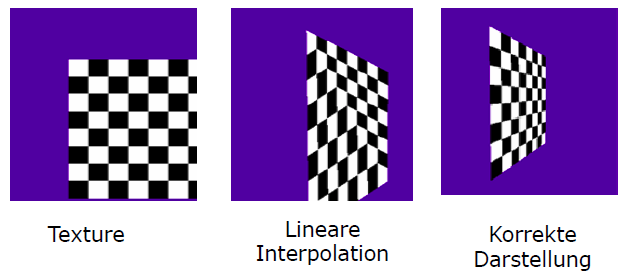
\includegraphics[width=0.4\linewidth]{fig/perspektive}
	\caption{Fehler bei der linearen Interpolation von Texturen}
	\label{fig:perspektive}
\end{figure}
Das hat den Ursprung darin, dass die Weltkoordinaten nicht die gleichen Abstände haben wie die Kamerakoordinaten. Das gute ist, dass diese perspektivische Korrektur in den heutigen Grafikkarten bereits vorimplementiert ist.

\section{Environment Mapping}
Man möchte z.B. die Umgebung in einem anderen Objekt spiegeln lassen. Dazu könnte man die gesamte Umgebung in 3D ebenfalls aufbauen und das Raytracing verwenden - was sehr ressourcenintensiv wäre. Andererseits könnte ja man einfach sich vorstellen, man ist im innern einer Kugel und projiziert auf dieses Innere eine Textur, welche dann die Umgebung darstellt. Somit vereinfacht sich die Berechnung der Umgebungsreflexion auf ein Objekt erheblich.
\begin{figure}[!ht]
	\centering
	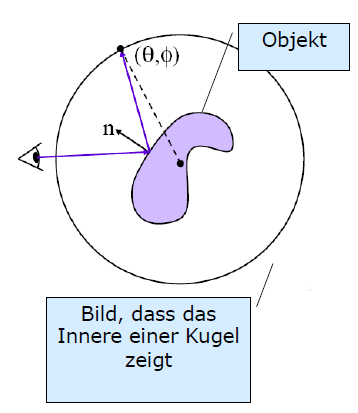
\includegraphics[width=0.4\linewidth]{fig/environment_mapping}
	\caption{Environment Mapping Beispiel}
	\label{fig:environment_mapping}
\end{figure}
\section{Bump Mapping}
Um eine etwas raue Oberfläche zu simulieren, könnte man tausende Polygone zusätzlich berechnen lassen - zu aufwändig. Daher verändert man einfach den Normalenvektor, mit dem man die Reflexionen des Lichts verändert zufällig.
\begin{figure}[!ht]
	\centering
	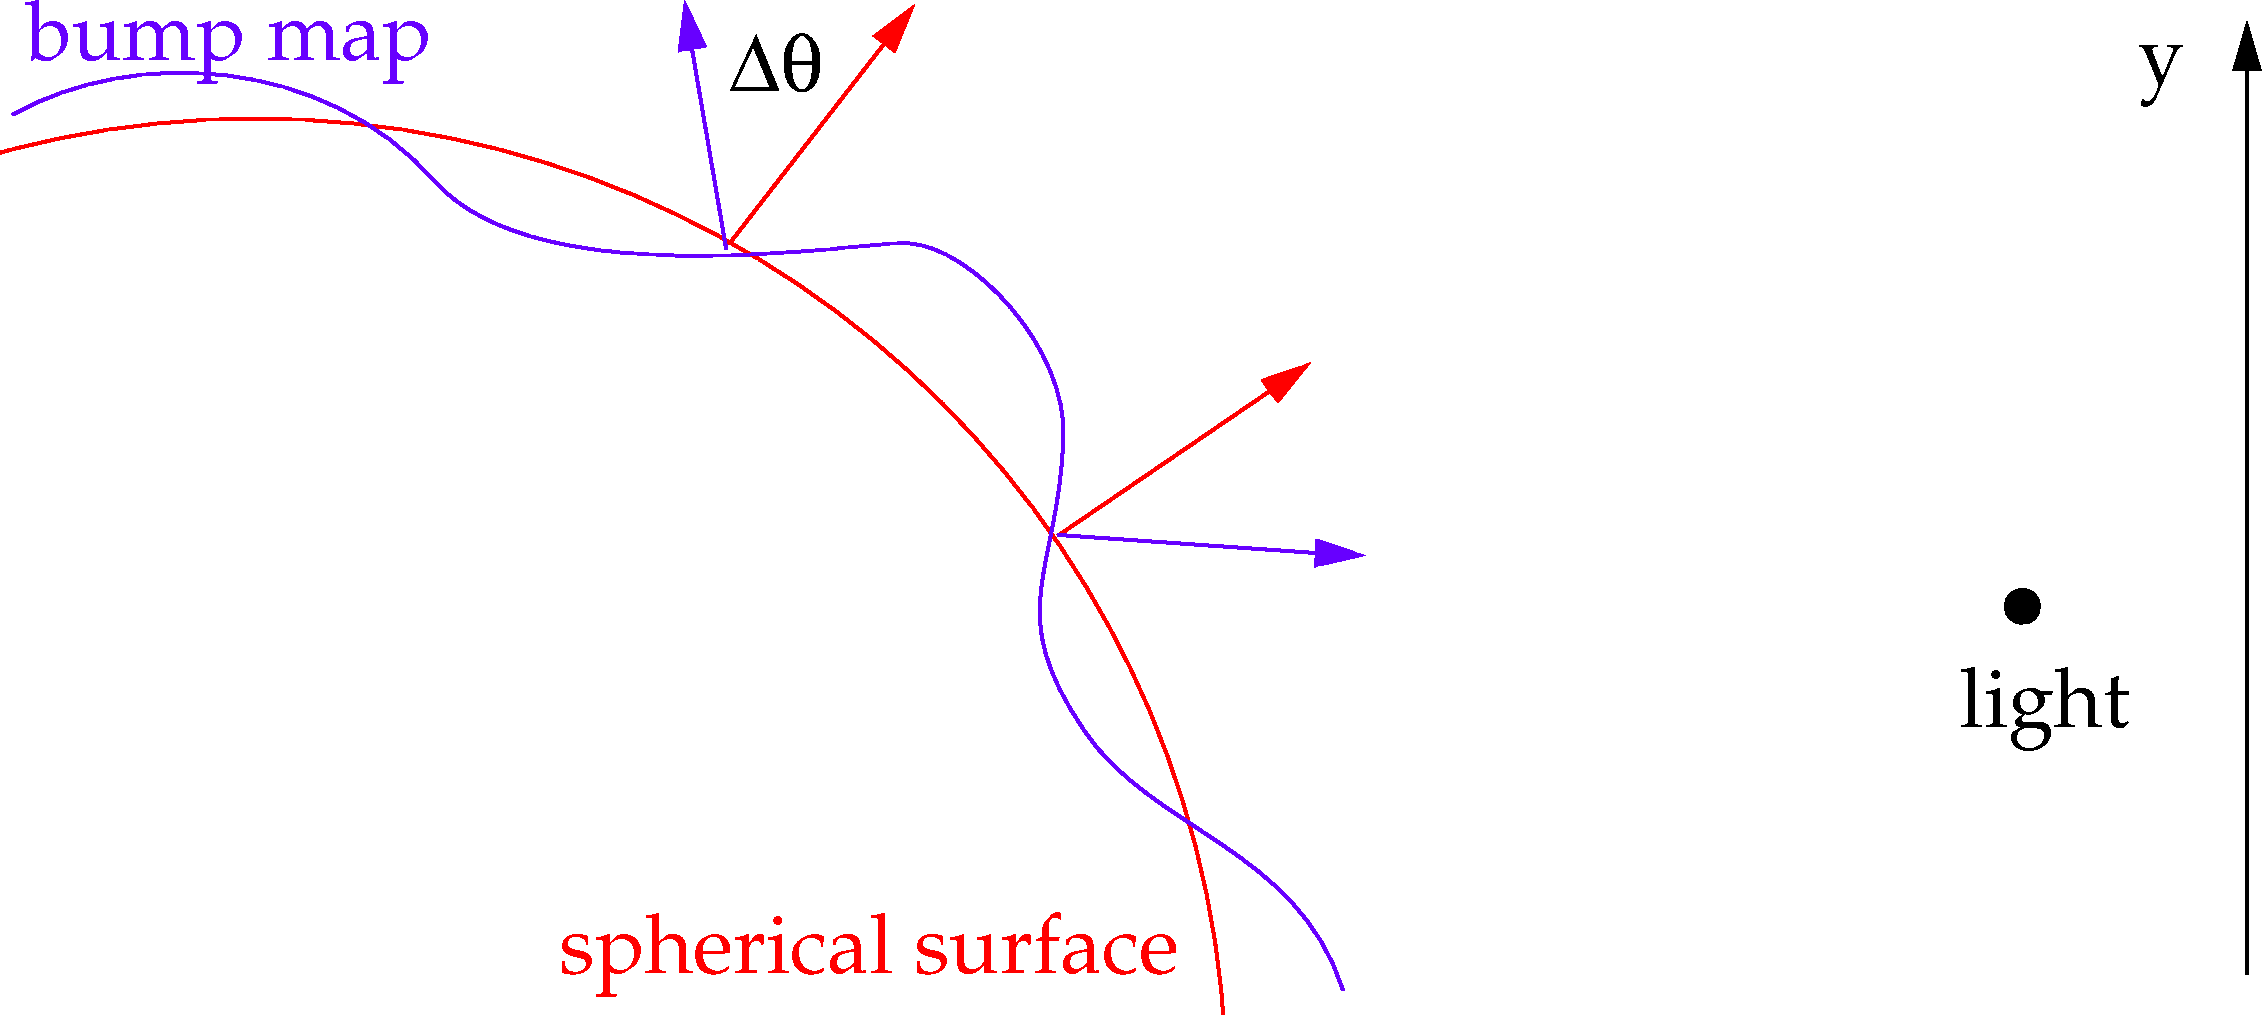
\includegraphics[width=0.4\linewidth]{fig/bumpmap}
	\caption{Bump Map Prinzip}
	\label{fig:bumpmap}
\end{figure}
\begin{figure}[!ht]
	\centering
	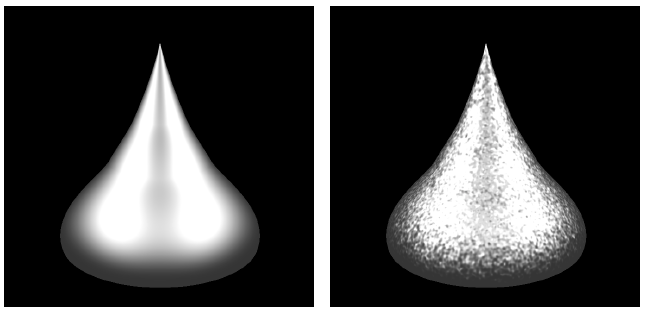
\includegraphics[width=0.4\linewidth]{fig/bumpmap_bsp}
	\caption{Bump Map Beispiel}
	\label{fig:bumpmap_bsp}
\end{figure}